\section{Conclusion}
\label{sec:conclusion}

In this fifth TCFE lab, we had to design a bandpass filter with an OP-AMP. Through mathematical tools such as OCTAVE, we were able to produce a theoretical analysis of the circuit and through NGSPICE we created a simulation of the circuit.

For the most part, there was not a significant difference between the theoretical results and the simulation results, so we have decided not to use a more acurate theoretical model of the OP-AMP, having instead chosen to maintain the ideal model. \par
However, the same cannot be said in regard to the phase response (Figure~\ref{fig:SIM_PH} or Figure~\ref{fig:CON_SIM_PH}). A possible explanation is the presence of two extra poles in the transfer function that are hidden in a more realistic OP-AMP, since there is a diference of $-180$ degrees to what would be expected if the transfer function~\ref{eq:T}.
Upon a closer inspection, the plot of the amplitude response (Figure~\ref{fig:SIM_OUT} or Figure~\ref{fig:CON_SIM_OUT}) does indicate the same two poles, one around $10^{4}$ Hz and $10^{6}$ Hz, that change de slope of the plot.
With this knowladge, we could, in theory, discart the low pass filter after the OP-AMP, and adjust the high pass filter accordingly. The problem with this approach is that we are not sure about the origin of additional low pass filter, or if it changes with input amplitude or other unknown paramaters.

The gain obtained by the two models was also different between simulation and theory, and the output impedance values were,as hinted in the beggining of this chapter, not very diferent from each other.

%%	Impedance

\begin{table}[h]
\centering
\begin{minipage}[t]{0.47\linewidth}
 	 \begin{tabular}[t]{|l|r|}
 	   \hline    
 	   {\bf Name} & {\bf Value} \\ \hline
 	   \input{../mat/MAT_IMP_tab}
 	 \end{tabular}
\end{minipage}
\begin{minipage}[t]{0.47\linewidth}
  	\begin{tabular}[t]{|l|r|}
    	\hline    
   		{\bf Name} & {\bf Value} \\ \hline
    	\input{../sim/SIM_ZIN_tab}
  	\end{tabular}
	\begin{tabular}[t]{|l|r|}
    	\hline    
   		{\bf Name} & {\bf Value [A or V]} \\ \hline
    	\input{../sim/SIM_ZOUT_tab}
  	\end{tabular}
\end{minipage}

\caption{Results in Octave and NGSpice, respectivily. NGSpice values are of of type {\it impedance} and expressed in Ohm; variables preceded by \# are of type {\it impedance} and expressed in Ohm; other variables are adimentional. (As shown in Tables \ref{tab:TEO_IMP}, \ref{tab:SIM_ZIN} and \ref{tab:SIM_ZOUT})}
\end{table}

%%	AC

\begin{table}[h]
\centering
\begin{minipage}[t]{0.40\linewidth}
 	 \begin{tabular}[t]{|l|r|}
 	   \hline    
 	   {\bf Name} & {\bf Value} \\ \hline
 	   \input{../mat/MAT_GAIN_tab}
 	 \end{tabular}
\end{minipage}
\begin{minipage}[t]{0.45\linewidth}
  	\begin{tabular}[t]{|l|r|}
    	\hline    
   		{\bf Name} & {\bf Value} \\ \hline
    	\input{../sim/SIM_DATA_tab}
  	\end{tabular}
\end{minipage}

  	\caption{Results in Octave and NGSpice, respectivily. Merit is in {\it per voltage per cost} and expressed in Volt$^{-1}$UC$^{-1}$; $f1 - f2$ is of the type {\it frequency} and expressed in Hz; amplitude ande amplitude - 100 are of the type {\it voltage} in Volt; other variables are adimentional. (As shown in Tables \ref{tab:TEO_RES} and \ref{tab:SIM_RES})}
\end{table}

The Merit result was $3.25*10^{-6}V^{-1}uc^{-1}$ by Ngspice. It was agreed by the members of the group that the main goal of task was completed, given the circunstances. 
We note that the main drives for the low figure of merit are two: the elevated cost of the OP-AMP and the lack of low resistors to use, as said in section~\ref{sec:analysis}.

\newpage
The obtained plot with NGSpice and Octave are the following:

\begin{figure}[h] \centering
	\vspace{-3cm}
	\includegraphics[height=12cm]{../sim/ampdb.pdf}
	\caption{NGSpice plot:$db(v_{out})$ and $max(db(v_{out}))-3$.}
	\label{fig:CON_MAT_OUT}
\end{figure}

\begin{figure}[h] \centering
	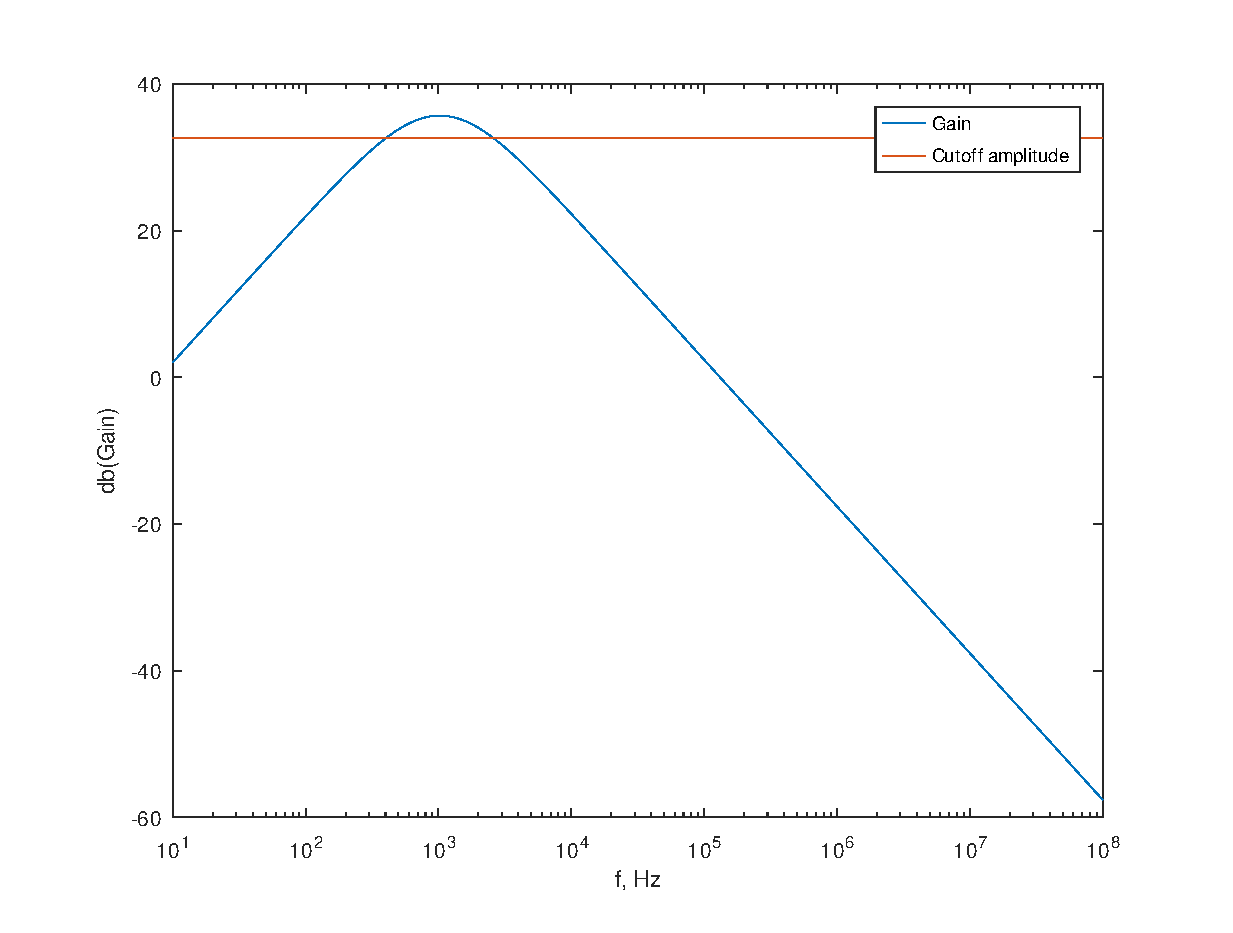
\includegraphics[height=8cm]{MAT_AB_AMP.eps}
	\caption{Octave plot:$db(v_{out})$ and $max(db(v_{out}))-3$.}
	\label{fig:CON_SIM_OUT}
\end{figure}

\newpage

\begin{figure}[h] \centering
	\vspace{-3cm}
	\includegraphics[height=12cm]{../sim/phdb.pdf}
	\caption{NGSpice plot: Phasor of $v_{out}$, rad}
	\label{fig:CON_MAT_PH}
\end{figure}

\begin{figure}[h] \centering
	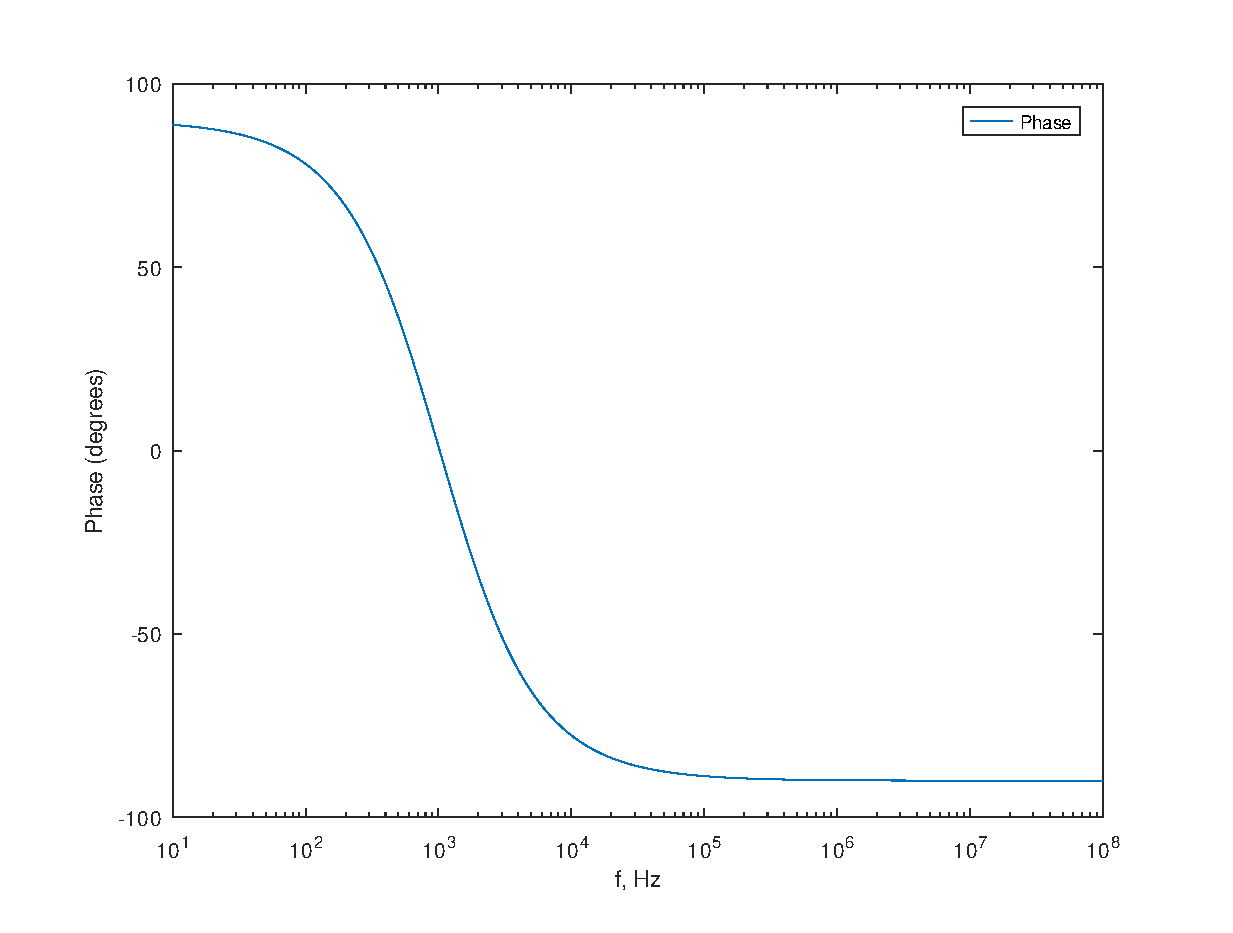
\includegraphics[height=8cm]{MAT_AB_PH.eps}
	\caption{Octave plot: Phasor of $v_{out}$, rad}
	\label{fig:CON_SIM_PH}
\end{figure}

\newpage

\begin{figure}[h] \centering
	\vspace{-3cm}
	\includegraphics[height=12cm]{../sim/trans.pdf}
	\caption{NGSpice plot: $v_{in}$ and $v_{out}$.}
	\label{fig:CON_SIM_TRANS}
\end{figure}
